% ŠABLONA PRO PSANÍ ZÁVĚREČNÉ STUDIJNÍ PRÁCE
%%%%%%%%%%%%%%%%%%%%%%%%%%%%%%%%%%%%%%%%%%%%
% Autor: Jakub Dokulil (kubadokulil99@gmail.com)
% Tato šablona byla vytvořena tak, aby pomocí ní mohli v systému LaTeX soutěžící sázet své práce a zároveň odpovídala požadavkům na formátování vyplývajícím z wordové šablony umístěné na webu soc.cz.
%
\documentclass[12pt, a4paper,
%oneside,      %% -- odkomentujte, pokud chcete svou práci mít pouze jednostrannou, mezera pro hřbet pak automaticky bude pouze na levé straně
twoside,        %% -- pro oboustranné práce, mezera pro hřbet následně střídá strany.
openright
]{report}

%% Nutné balíčky a nastavení
%%%%%%%%%%%%%%%%%%%%%%%%%%%%

%% Proměnné
\newcommand\obor{INFORMAČNÍ TECHNOLOGIE} %% -- napiš číslo a název tvého oboru
\newcommand\kodOboru{18-20-M/01} %% -- napiš číslo a název tvého oboru
\newcommand\zamereni{se zaměřením na počítačové sítě a programování} %% -- napiš číslo a název tvého oboru
\newcommand\skola{Střední škola průmyslová a umělecká, Opava} %% vyplň název školy
\newcommand\trida{IT4} %% vyplň jméno svého konzultanta
\newcommand\jmenoAutora{Lukáš Hrňa}  %% vyplň své jméno
\newcommand\skolniRok{2023/24} %% vyplň rok
\newcommand\datumOdevzdani{1. 1. 2024} %% vyplň rok
\newcommand\nazevPrace{NeuralPath Labyrinth} %% vyplň název své práce

\title{\nazevPrace} %% -- Název tvé práce
\author{\jmenoAutora} %% -- tvé jméno
\date{\datumOdevzdani} %% -- rok, kdy píšeš SOČku

\usepackage[top=2.5cm, bottom=2.5cm, left=2.5cm, right=2.5cm]{geometry}
\usepackage{float}

\usepackage[czech]{babel} %% balík babel pro sazbu v češtině
\usepackage[utf8]{inputenc} %% balíky pro kódování textu
\usepackage[T1]{fontenc}
\usepackage{cmap} %% balíček zajišťující, že vytvořené PDF bude prohledávatelné a kopírovatelné

\usepackage{graphicx} %% balík pro vkládání obrázků

\usepackage{subcaption} %% balíček pro vkládání podobrázků

\usepackage{hyperref} %% balíček, který v PDF vytváří odkazy

\linespread{1.25} %% řádkování
\setlength{\parskip}{0.5em} %% odsazení mezi odstavci


\usepackage[pagestyles]{titlesec} %% balíček pro úpravu stylu kapitol a sekcí
\titleformat{\chapter}[block]{\scshape\bfseries\LARGE}{\thechapter}{10pt}{\vspace{0pt}}[\vspace{-22pt}]
\titleformat{\section}[block]{\scshape\bfseries\Large}{\thesection}{10pt}{\vspace{0pt}}
\titleformat{\subsection}[block]{\bfseries\large}{\thesubsection}{10pt}{\vspace{0pt}}


\usepackage{tocloft} % Balíček umožní přizpůsobit vzhled tabulky obsahu
\setlength{\cftbeforechapskip}{0pt}  % Menší rozestup pro kapitoly
\setlength{\cftbeforesecskip}{0pt}   % Menší rozestup pro sekce

\setcounter{secnumdepth}{2}
\setcounter{tocdepth}{1}
\usepackage{fancyhdr}
\pagestyle{fancy}
\fancyhf{} % Vymaže obsah záhlaví a zápatí
\fancyhead{} % Vymaže obsah záhlaví (včetně názvů kapitol)
\fancyfoot[C]{\thepage} % Umístí číslo stránky do středu zápatí
\renewcommand{\headrulewidth}{0pt} % Odstraní horizontální čáru v záhlaví
\renewcommand{\footrulewidth}{0pt} % Odstraní horizontální čáru v zápatí

\pagestyle{fancy}
\renewcommand{\headrulewidth}{0.025pt}

\usepackage{booktabs}

\usepackage{url}

%% Balíčky co se můžou hodit :) 
%%%%%%%%%%%%%%%%%%%%%%%%%%%%%%%

\usepackage{pdfpages} %% Balíček umožňující vkládat stránky z PDF souborů, 

\usepackage{upgreek} %% Balíček pro sazbu stojatých řeckých písmen, třeba u jednotky mikrometr. Například stojaté mí: \upmu, stojaté pí: \uppi

\usepackage{amsmath}    %% Balíčky amsmath a amsfonts 
\usepackage{amsfonts}   %% pro sazbu matematických symbolů
\usepackage{esint}     %% pro sazbu různých integrálů (např \oiint)
\usepackage{mathrsfs}
\usepackage{helvet} % Helvet font
\usepackage{mathptmx} % Times New Roman
\usepackage{Oswald} % Oswald font


%% makra pro sazbu matematiky
\newcommand{\dif}{\mathrm{d}} %% makro pro sazbu diferenciálu, místo toho
%% abych musel psát '\mathrm{d}' mi stačí napsat '\dif' což je mnohem 
%% kratší a mohu si tak usnadnit práci

\usepackage{listings}
\usepackage{xcolor}

\renewcommand{\lstlistingname}{Kód}% Listing -> Algorithm
\renewcommand{\lstlistlistingname}{Seznam programových kódů}% List of Listings -> List of Algorithms

\definecolor{GrayCodeBlock}{RGB}{241,241,241}
\definecolor{BlackText}{RGB}{110,107,94}
\definecolor{RedTypename}{RGB}{182,86,17}
\definecolor{GreenString}{RGB}{96,172,57}
\definecolor{PurpleKeyword}{RGB}{184,84,212}
\definecolor{GrayComment}{RGB}{170,170,170}
\definecolor{GoldDocumentation}{RGB}{180,165,45}
\lstdefinelanguage{rust}
{
	columns=fullflexible,
	keepspaces=true,
	frame=single,
	framesep=0pt,
	framerule=0pt,
	framexleftmargin=4pt,
	framexrightmargin=4pt,
	framextopmargin=5pt,
	framexbottommargin=3pt,
	xleftmargin=4pt,
	xrightmargin=4pt,
	backgroundcolor=\color{GrayCodeBlock},
	basicstyle=\ttfamily\color{BlackText},
	keywords={
		true,false,
		unsafe,async,await,move,
		use,pub,crate,super,self,mod,
		struct,enum,fn,const,static,let,mut,ref,type,impl,dyn,trait,where,as,
		break,continue,if,else,while,for,loop,match,return,yield,in
	},
	keywordstyle=\color{PurpleKeyword},
	ndkeywords={
		bool,u8,u16,u32,u64,u128,i8,i16,i32,i64,i128,char,str,
		Self,Option,Some,None,Result,Ok,Err,String,Box,Vec,Rc,Arc,Cell,RefCell,HashMap,BTreeMap,
		macro_rules
	},
	ndkeywordstyle=\color{RedTypename},
	comment=[l][\color{GrayComment}\slshape]{//},
	morecomment=[s][\color{GrayComment}\slshape]{/*}{*/},
	morecomment=[l][\color{GoldDocumentation}\slshape]{///},
	morecomment=[s][\color{GoldDocumentation}\slshape]{/*!}{*/},
	morecomment=[l][\color{GoldDocumentation}\slshape]{//!},
	morecomment=[s][\color{RedTypename}]{\#![}{]},
	morecomment=[s][\color{RedTypename}]{\#[}{]},
	stringstyle=\color{GreenString},
	string=[b]"
}




%% Definice 
\lstdefinelanguage{JavaScript}{
	morekeywords=[1]{break, continue, delete, else, for, function, if, in,
		new, return, this, typeof, var, void, while, with},
	% Literals, primitive types, and reference types.
	morekeywords=[2]{false, null, true, boolean, number, undefined,
		Array, Boolean, Date, Math, Number, String, Object},
	% Built-ins.
	morekeywords=[3]{eval, parseInt, parseFloat, escape, unescape},
	sensitive,
	morecomment=[s]{/*}{*/},
	morecomment=[l]//,
	morecomment=[s]{/**}{*/}, % JavaDoc style comments
	morestring=[b]',
	morestring=[b]"
}[keywords, comments, strings]


\lstdefinelanguage[ECMAScript2015]{JavaScript}[]{JavaScript}{
	morekeywords=[1]{await, async, case, catch, class, const, default, do,
		enum, export, extends, finally, from, implements, import, instanceof,
		let, static, super, switch, throw, try},
	morestring=[b]` % Interpolation strings.
}

\lstalias[]{ES6}[ECMAScript2015]{JavaScript}

% Nastavení barev
% Requires package: color.
\definecolor{mediumgray}{rgb}{0.3, 0.4, 0.4}
\definecolor{mediumblue}{rgb}{0.0, 0.0, 0.8}
\definecolor{forestgreen}{rgb}{0.13, 0.55, 0.13}
\definecolor{darkviolet}{rgb}{0.58, 0.0, 0.83}
\definecolor{royalblue}{rgb}{0.25, 0.41, 0.88}
\definecolor{crimson}{rgb}{0.86, 0.8, 0.24}

% Nastavení pro Python
\lstdefinestyle{Python}{
	language=Python,
	backgroundcolor=\color{white},
	basicstyle=\ttfamily,
	breakatwhitespace=false,
	breaklines=false,
	captionpos=b,
	columns=fullflexible,
	commentstyle=\color{mediumgray}\upshape,
	emph={},
	emphstyle=\color{crimson},
	extendedchars=true,  % requires inputenc
	fontadjust=true,
	frame=single,
	identifierstyle=\color{black},
	keepspaces=true,
	keywordstyle=\color{mediumblue},
	keywordstyle={[2]\color{darkviolet}},
	keywordstyle={[3]\color{royalblue}},
	literate=%
	{á}{{\'a}}1 {č}{{\v{c}}}1 {ď}{{\v{d}}}1 {é}{{\'e}}1 {ě}{{\v{e}}}1
	{í}{{\'i}}1 {ň}{{\v{n}}}1 {ó}{{\'o}}1 {ř}{{\v{r}}}1 {š}{{\v{s}}}1
	{ť}{{\v{t}}}1 {ú}{{\'u}}1 {ů}{{\r{u}}}1 {ý}{{\'y}}1 {ž}{{\v{z}}}1,		
	numbers=left,
	numbersep=5pt,
	numberstyle=\tiny\color{black},
	rulecolor=\color{black},
	showlines=true,
	showspaces=false,
	showstringspaces=false,
	showtabs=false,
	stringstyle=\color{forestgreen},
	tabsize=2,
	title=\lstname,
	upquote=true  % requires textcomp	
}


\lstdefinestyle{JSES6Base}{
	backgroundcolor=\color{white},
	basicstyle=\ttfamily,
	breakatwhitespace=false,
	breaklines=false,
	captionpos=b,
	columns=fullflexible,
	commentstyle=\color{mediumgray}\upshape,
	emph={},
	emphstyle=\color{crimson},
	extendedchars=true,  % requires inputenc
	fontadjust=true,
	frame=single,
	identifierstyle=\color{black},
	keepspaces=true,
	keywordstyle=\color{mediumblue},
	keywordstyle={[2]\color{darkviolet}},
	keywordstyle={[3]\color{royalblue}},
 literate=%
{á}{{\'a}}1 {č}{{\v{c}}}1 {ď}{{\v{d}}}1 {é}{{\'e}}1 {ě}{{\v{e}}}1
{í}{{\'i}}1 {ň}{{\v{n}}}1 {ó}{{\'o}}1 {ř}{{\v{r}}}1 {š}{{\v{s}}}1
{ť}{{\v{t}}}1 {ú}{{\'u}}1 {ů}{{\r{u}}}1 {ý}{{\'y}}1 {ž}{{\v{z}}}1,		
	numbers=left,
	numbersep=5pt,
	numberstyle=\tiny\color{black},
	rulecolor=\color{black},
	showlines=true,
	showspaces=false,
	showstringspaces=false,
	showtabs=false,
	stringstyle=\color{forestgreen},
	tabsize=2,
	title=\lstname,
	upquote=true  % requires textcomp
}

\lstdefinestyle{JavaScript}{
	language=JavaScript,
	style=JSES6Base,
}
\lstdefinestyle{ES6}{
	language=ES6,
	style=JSES6Base
}


%% Začátek dokumentu
%%%%%%%%%%%%%%%%%%%%
\begin{document}
	
	\pagestyle{fancy}
	\pagenumbering{Roman}
	
	\cleardoublepage

%% Titulní stránka s informacemi
%%%%%%%%%%%%%%%%%%%%%%%%%%%%%%%%%%%%%%%%
	
	{\fontfamily{phv}\selectfont
		%% Logo školy
		\begin{figure}[h]
			\centering
			
\includegraphics[width=0.6\linewidth]{image/logo-skoly.png} 
		\end{figure}
		
		
		%% Hlavička práce a její název (viz proměnná \nazev prace)
		%% \sffamily %%% bezpatkové písmo - sans serif
		{\bfseries %%% písmo na stránce je tučně
			\begin{center}
				\vspace{0.025 \textheight}
				\LARGE{ZÁVĚREČNÁ STUDIJNÍ PRÁCE}\\
				\large{dokumentace}\\
				\vspace{0.075 \textheight}
				\LARGE {\nazevPrace}\\
			\end{center}  
		}%%%
		
		\begin{figure}[h]
			\centering
			
\includegraphics[width=0.7\linewidth]{image/programovani-02.jpeg} 
		\end{figure}
		
		\vspace{0.02 \textheight}
		\begin{table}[h!]
			\begin{tabular}{ll}
				\textbf{Autor:} & \jmenoAutora\\ 
				\textbf{Obor:} & \kodOboru { } \obor\\
				\textbf{} & \zamereni\\
				\textbf{Třída:} & \trida\\
				\textbf{Školní rok:} & \skolniRok\\
			\end{tabular}
			
		\end{table}		
	}
	
\cleardoublepage %% Zalomení dvojstránky
	
%% Stránka obsahující poděkování a prohlášení
%%%%%%%%%%%%%%%%%%%%%%%%%%%%%%%%%%%%%%%%%%%%%%%%%%%%%%%%

%% Poděkování - nepovinné
%%%%%%%%%%%%%%%%%%%%%%%%%%%%
	
	\noindent{\large{\bfseries{Poděkování}\\}}
	\noindent Prostor k poděkování Tučňákovi.
	
	\vspace*{0.7\textheight} %% Vertikální mezeru je možné upravit

%% Prohlášení - povinné
%%%%%%%%%%%%%%%%%%%%%%%%%%%%
	\noindent{\large{\bfseries{Prohlášení}\\}}  %% uprav si koncovky podle toho na jaký rod se cítíš, vypadá to pak lépe :) 
	\noindent{Prohlašuji, že jsem závěrečnou práci vypracoval samostatně a uvedl veškeré použité 
		informační zdroje.\\}
	\noindent{Souhlasím, aby tato studijní práce byla použita k výukovým a prezentačním účelům na Střední průmyslové a umělecké škole v Opavě, Praskova 399/8.}
	\vfill
	\noindent{V Opavě \datumOdevzdani\\}
	\noindent
	\begin{minipage}{\linewidth}
		\hspace{9.5cm} 
		\begin{tabular}{@{}p{6cm}@{}}
			\dotfill \\
			Podpis autora
		\end{tabular}
	\end{minipage}
	
	\cleardoublepage %% Zalomení dvojstránky

%% Stránka obsahující abstrakt (anotaci)
%%%%%%%%%%%%%%%%%%%%%%%%%%%%%%%%%%%%%%%%%%%%%%%%%%%%%%%%	

%% Abstrakt v češtině
%%%%%%%%%%%%%%%%%%%%%%%%%%%%
\noindent{\Large{\bfseries{Abstrakt}\\}}
\noindent Tento projekt se zaměřuje na aplikaci umělé inteligence pro řešení jednoduchých bludišť. Využíváme PyTorch, knihovnu pro strojové učení, nástroj pro vývoj a testování algoritmů posilovaného učení. Cílem je vyvinout a trénovat model AI, který efektivně prochází prostředím generovaných bludišť. Model je navržen pro rozpoznávání vzorů a navigaci různými konfiguracemi bludišť s cílem najít cestu ven.

\vspace{18pt}

\noindent{\large{\bfseries{Klíčová slova}}}

\noindent Umělá inteligence, Posilované učení, PyTorch, Navigace bludištěm, Hluboké neuronové sítě, Prostorová navigace, Algoritmy pro hledání cesty, Generování bludišť
\vspace{18pt}

%% Abstrakt v angličtině
%%%%%%%%%%%%%%%%%%%%%%%%%%%%    
\noindent{\Large{\bfseries{Abstract}}}

\noindent This project focuses on the application of artificial intelligence to solve simple mazes. We utilize PyTorch, a machine learning library, a tool for developing and testing reinforcement learning algorithms. The goal is to develop and train an AI model capable of efficiently navigating through the environment of generated mazes. The model is designed to recognize patterns and navigate through various maze configurations to find a way out.

\vspace{18pt}

\noindent{\large{\bfseries{Keywords}}}

\noindent Artificial Intelligence, Reinforcement Learning, PyTorch, Maze Navigation, Neural Networks, Spatial Navigation, Pathfinding Algorithms, Maze Generation 

\clearpage %% Zalomení stránky

%% Stránka s generovaným obsahem
%%%%%%%%%%%%%%%%%%%%%%%%%%%%%%%%%%%%%%%    

\tableofcontents %% Vygeneruje tabulku s obsahem

\pagenumbering{arabic} %% Nastavení způsobu číslování stránek (alternativy roman | Roman)
\setcounter{page}{1} %% Nastavení počitadla stránek

%% Stránka s úvodem - povinná část
%%%%%%%%%%%%%%%%%%%%%%%%%%%%%%%%%%%%%%%        
\chapter*{Úvod}
\addcontentsline{toc}{chapter}{Úvod}
V této závěrečné studijní práci se věnujeme fascinujícímu tématu aplikace umělých neuronových sítí v prostředí 2D bludiště. Cílem práce je prozkoumat a demonstrovat, jak mohou technologie umělé inteligence, zejména neuronové sítě, efektivně řešit složité úlohy navigace a rozhodování v dynamických a neznámých prostředích.

Zaměřujeme se především na teoretické základy neuronových sítí, včetně jejich struktury, typů učení a klíčových algoritmů, jako je Q-learning a jeho rozšíření v Deep Q-networks. Tyto metody poskytují základní rámec pro porozumění tomu, jak AI modely zpracovávají informace, učí se z získaných dat a adaptují se na nové situace v prostředí bludiště.

Praktická část práce zahrnuje vývoj vlastního 2D bludiště, které slouží jako testovací prostředí pro umělou inteligenci. Využíváme programovací jazyk Rust pro generování bludiště a Python s knihovnami jako PyTorch pro vývoj a trénování AI modelu. Dále popisujeme, jakým způsobem AI interaguje s bludištěm, jaké metody a nástroje jsou využívány pro sledování a zaznamenávání jejího chování a jaké výzvy tento proces přináší.



%Tipy k psaní úvodu
%Je povinný, nadpis neměňte, rozsah - max. 1 strana. 
%Tato část práce obsahuje: 
%* náhled do řešené problematiky, zdůvodnění volby problematiky, 
%* předem definované cíle práce, 
%* motivaci pro další čtení textu včetně stručného uvedení obsahu následujících kapitol 


\chapter{Umělé Neuronové Sítě}

\section{Úvod}
\label{sec:uvod}

Tato kapitola slouží jako úvod do tématu umělých neuronových sítí. Zabývá se vysvětlením základních pojmů, popisem matematického modelu neuronu a jeho schopností klasifikace. Klíčovým prvkem je pochopení matematického modelu jednoho neuronu, což je základ pro pochopení komplexnějších struktur tvořených propojenými neurony v rámci umělých neuronových sítí



\section{Typy učení}
\label{sec:prace_s_textem}
Učení v umělé inteligenci lze rozdělit do několika základních kategorií, z nichž nejvýznamnější jsou učení s učitelem, bez učitele a posilované učení. Každý typ má své specifické charakteristiky a využití.

\subsection{Unsupervised learning}
Učení bez učitele, nebo unsupervised learning, pracuje s neoznačenými daty. Cílem je najít skryté vzory nebo struktury v datech, aniž by byly k dispozici předem definované odpovědi nebo labely. Typickými příklady využití jsou klastrování, kde je úkolem najít skupiny podobných prvků v datech, nebo redukce dimenzionality, která slouží k zjednodušení komplexních datových sad. Učení bez učitele je klíčové v situacích, kdy je třeba rozpoznat inherentní strukturu dat bez předchozích znalostí o tom, co data přesně obsahují.
\begin{figure}[h]
	\centering
	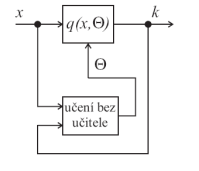
\includegraphics{image/bezu.png} 
\end{figure}

\subsection{Supervised learning}
Učení s učitelem, nebo supervised learning, je proces, kde model umělé inteligence je trénován na datové sadě, která obsahuje jak vstupní data, tak správné odpovědi (labely). Tento přístup umožňuje modelu naučit se předpovídat výstupy na základě nových vstupů na základě předchozích zkušeností. Tento typ učení je široce využíván v aplikacích jako je klasifikace (například rozpoznávání objektů na obrázcích) a regrese (například předpovídání cen nemovitostí), kde je důležité, aby model byl schopen správně identifikovat a reagovat na různé druhy dat.
\begin{figure}[h]
	\centering
	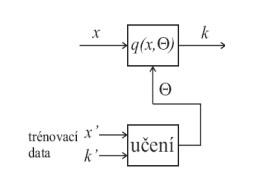
\includegraphics{image/su.png} 
\end{figure}


\subsection{Reinforcement learning}
Posilované učení, nebo reinforcement learning, je zase odlišné tím, že se zaměřuje na vývoj algoritmů, které se učí prostřednictvím interakce s prostředím a získávají zpětnou vazbu v podobě odměn nebo trestů. V tomto přístupu je agent, kterým může být například robot nebo software, vystaven prostředí, ve kterém se snaží provádět akce vedoucí k maximální možné odměně. Posilované učení je ideální pro situace, kde jsou rozhodnutí časově závislá a kde je třeba vzít v úvahu dlouhodobé důsledky akcí, jako jsou strategické hry, robotická navigace nebo autonomní řízení vozidel.
\begin{figure}[h]
	\centering
	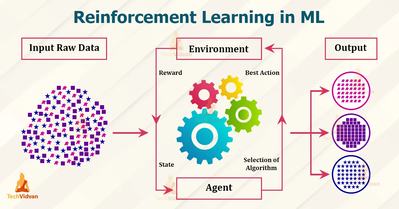
\includegraphics[width=0.8\linewidth, height=0.8\linewidth, keepaspectratio]{image/reinu.png}
	
\end{figure}

Pro maximalizaci celkové odměny je nezbytné, aby agent volil optimální akce v závislosti na svém současném stavu. Tento výběr akcí, známý jako strategie nebo politika $\pi$
, je klíčový pro přiřazení nejvhodnější akce pro každý stav. Existuje mnoho algoritmů pro určení efektivní funkce $\pi$
, nicméně zde se zaměříme specificky na Q-learning a jeho odvozené algoritmy.




\section{Q-learning}

Q-learning je algoritmus založený na principu posilovaného učení. Na rozdíl od metod, které přímo hledají optimální strategii $\pi$ (metody policy gradient), Q-learning postupuje nepřímo prostřednictvím tzv. Q-tabulky. Tato tabulka spojuje stavy s akcemi - každý řádek reprezentuje jeden stav a sloupce v tomto řádku různé akce. Agent vybírá akci s nejvyšší hodnotou v tabulce. Tyto hodnoty jsou známé jako Q-hodnoty, kde "Q" reprezentuje "quality" (kvalitu) akce. Algoritmus, který určuje nejlepší akci z Q-tabulky, je označován jako Q-funkce.
\begin{figure}[h]
	\centering
	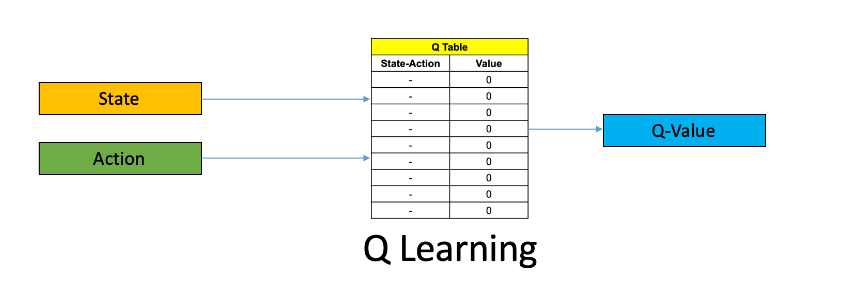
\includegraphics[width=0.8\linewidth, height=0.8\linewidth, keepaspectratio]{image/qlearn2.png}
	
\end{figure}
Aktualizace Q-hodnot se provádí na základě odměn, které agent obdrží od prostředí za provedenou akci. Tato odměna, známá jako posílení, může být pozitivní, negativní (trest) nebo neutrální. Když agent obdrží za určitou akci negativní odměnu, dojde k snížení příslušné hodnoty v Q-tabulce, což vede k nižší pravděpodobnosti opětovného výběru této akce. Takto lze postupně eliminovat nežádoucí chování a podporovat chování, které je žádoucí.

\subsection{Okamžitá a dlouhodobá odměna}
Aktualizace Q-hodnot lze rozdělit na dvě zásadní části: okamžitou a dlouhodobou. Okamžitá část je reprezentována odměnou $r_{t}$, kterou agent obdrží za provedení akce $a_{t}$. K této okamžité odměně je pak přičítána dlouhodobá hodnota, reprezentující očekávané budoucí Q-hodnoty ze stavu $s_{t+1}$. Cílem je maximalizovat celkovou odměnu, zahrnující nejen aktuální, ale i budoucí akce. Například, v případě dvou možných akcí ($a_{1}$, $a_{2}$) ve stavu $s_{0}$ může být na první pohled akce s vyšší okamžitou odměnou méně výhodná v dlouhodobém horizontu, pokud by v důsledku jejího provedení následovaly stavy vedoucí k nižším celkovým odměnám.

\begin{figure}[h]
	\centering
	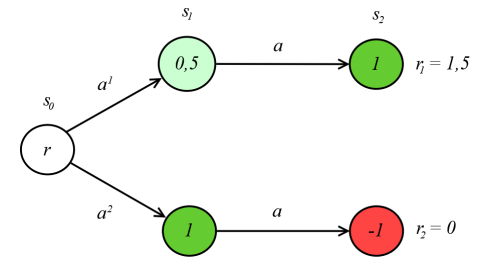
\includegraphics[width=0.8\linewidth, height=0.8\linewidth, keepaspectratio]{image/odmen.png}
\end{figure}[h]

Je klíčové najít správnou rovnováhu mezi okamžitou a dlouhodobou odměnou. Úloha dlouhodobé odměny může být upravena pomocí diskontního faktoru (discount factor) \(\gamma\), který určuje váhu budoucích odměn, zatímco míra učení (learning rate) \(\alpha\) ovlivňuje rychlost aktualizace Q-hodnot. Celkovou odměnu \(r\), skládající se z okamžité a dlouhodobé složky, lze vyjádřit jako součet těchto dvou komponent, s přihlédnutím k váze diskontního faktoru a míry učení.

\begin{equation}
	r=a.(r_{t}+\gamma . maxQ(s_{t+1,a}))
\end{equation}



V Q-tabulce se Q-hodnota pro daný stav a akci obvykle nepřepisuje přímo novou odměnou, ale upravuje se na základě již existující hodnoty. Toto se provádí za účelem zachování historických informací o výkonnosti dané akce. Aktualizační pravidlo pro Q-hodnoty tedy bude kombinovat aktuální odměnu s předešlými poznatky o daném stavu a akci, čímž se dosahuje efektivnějšího a přesnějšího učení.

\begin{equation}
	Q^{nova}(s_t,a_t)=(1-\alpha).Q(s_{t},a{t})+r
\end{equation}

\newpage
\subsection{Limitace Q-learningu}
Při použití Q-tabulky pro mapování stavů na akce v rámci Q-learningu se můžeme setkat s několika komplikacemi. Pro složitější úlohy, kde je stav určen několika proměnnými současně (například v 3D prostoru), může velikost Q-tabulky dosáhnout extrémních rozměrů, což vede k její nepraktičnosti. Navíc, protože stavy musí tvořit konečnou sadu, řešení spojitých stavů se stává problematickým. Další výzvou je manipulace s akcemi: v základním modelu Q-learningu jsou akce pouze přijaty nebo odmítnuty (binární výběr), což znemožňuje spojité řízení výstupu. Tyto problémy mohou být řešeny implementací umělých neuronových sítí, které nabízí flexibilnější a efektivnější přístup.



\newpage
\subsection{Deep Q-network}

Deep Q-network (DQN) je algoritmus, který byl vytvořen společností DeepMind v roce 2015. Tento algoritmus spojuje principy Q-learningu s umělou neuronovou sítí. Základním konceptem DQN je využití neuronové sítě, známé jako Q-síť, která nahrazuje tradiční Q-tabulku. Úkolem této sítě je co nejvíce přiblížit funkci Q-hodnoty. Vstupem do Q-sítě je stav $s_{t}$, a výstupem je reakce na tento stav $a_{t}$, což je podobné Q-tabulce. Nicméně, proces učení Q-sítě se liší od Q-tabulky, protože zde nelze jednoduše aktualizovat Q-hodnoty. Místo toho se Q-síť musí učit stejným způsobem jako jakákoliv jiná neuronová síť, a to využitím učení s učitelem, kde jsou všechny akce agenta stále hodnoceny pomocí odměňovací funkce a generují trénovací data.

Další rozdíl oproti klasickému Q-learningu je v aktualizačním pravidle. Vzhledem k tomu, že neuronovou síť neměníme přímo, vynecháváme část aktualizačního pravidla, která připočítává starou Q-hodnotu. Toto pravidlo aktualizace pak nabývá nové formy, která efektivně využívá schopnosti neuronové sítě k učení a přizpůsobení.

\begin{equation}
  Q^{nova}(s_t,a_t)=r_t+\gamma maxQ(s_{t+1},a)
\end{equation}


Neuronové sítě jsou efektivnější, když se učí na základě více dat, než jen jednoho výstupu. Efektivnějším přístupem je uchovávání historie předchozích stavů agenta. Zaznamenáváme stav, akci, odměnu a následující stav ($s_{t}$, $a_{t}$, $r_{t}$, $s_{t+1}$) - všechny elementy potřebné pro výpočet nových Q-hodnot. Během učení pak agent vybírá náhodně uspořádanou vzorku pevně stanovené velikosti z těchto uložených záznamů. Na základě této vzorky se počítají nové Q-hodnoty, které jsou poté uplatněny na neuronovou síť pomocí algoritmu zpětného šíření chyb. Tento proces uchovávání minulých stavů se nazývá metoda opakování zkušeností (experience replay).

\begin{figure}[h]
	\centering
	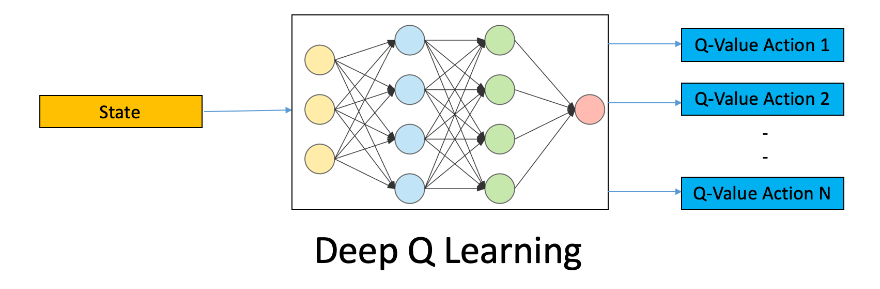
\includegraphics[width=0.8\linewidth, height=0.8\linewidth, keepaspectratio]{image/dqlearn.png}
	
\end{figure}

\newpage
\section{Perceptron}
Perceptron v nejjednodušší podobě je binární klasifikátor, který mapuje vektory vstupů 
\(\mathbf{x} = [x_1, x_2, \ldots, x_n]\) na výstupní hodnoty \(f(\xi)\):
\[
f(\xi) = 
\begin{cases} 
	1 & \text{pro } \mathbf{w} \cdot \mathbf{x} - \theta \geq 0 \\
	0 & \text{jindy} 
\end{cases}
\]
kde \(\mathbf{w}\) je vektor vah a \(\theta\) je práh citlivosti neuronu.

Celkový podnět neuronu udává vážený součet \(\xi = \sum_{i=1}^{n} w_i \cdot x_i - \theta\). Tento celkový podnět bývá označován jako potenciál neuronu. Na potenciál reaguje neuron (perceptron) výstupní odezvou \(Z = f(\xi)\), kde \(f\) je tzv. přenosová funkce. Je-li přenosová funkce ve tvaru skokové funkce, perceptron funguje, jak již bylo řečeno, jako binární klasifikátor, neuron tedy dělí vstupní prostor na dvě části.
\begin{figure}[h]
	\centering
	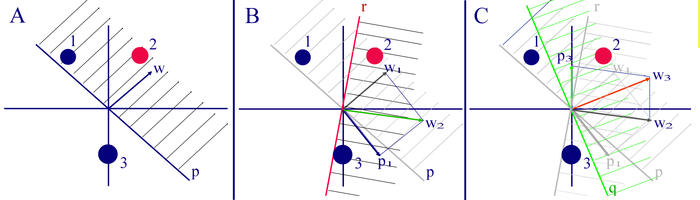
\includegraphics[width=0.8\linewidth, height=0.8\linewidth, keepaspectratio]{image/tri.png}
	
\end{figure}
Tři fáze učení jednoduchého perceptronu jsou následující:

\begin{enumerate}
	\item[A:] Je zvolen náhodně vektor vah \(\mathbf{w}\) a k němu určena kolmá rozhodovací hranice \(p\). Zjišťujeme výstup pro bod 1 - leží v oblasti s výstupem 1, i když má ležet v oblasti s výstupem 0. 
	\item[B:] Odečteme vektor bodu 1 od vektoru vah \(\mathbf{w_1}\) a získáme nový vektor vah \(\mathbf{w_2}\) a k němu příslušnou rozhodovací hranici znázorněnou přímkou \(r\). Bod 2 je umístěn správně, bodu 3 přiřadí síť hodnotu 1 i když má dostat výstup 0.
	\item[C:] Odečteme vektor bodu 3 od vektoru vah \(\mathbf{w_2}\) a získáme nový vektor vah \(\mathbf{w_3}\). Nyní je již problém vyřešen - všem bodům je přiřazen odpovídající hodnota výstupu. Řešením problému je tedy vektor vah \(\mathbf{w_3}\) s příslušnou rozhodovací hranicí \(q\).
\end{enumerate}



\newpage
\section{Multi layer perceptron(MLP)}

MLP je rozšířením dopředné neuronové sítě. Skládá se ze tří typů vrstev - vstupní vrstvy, výstupní vrstvy a skrytých vrstev. Vstupní vrstva přijímá vstupní signál k zpracování. Výstupní vrstva provádí požadované úlohy, jako jsou predikce a klasifikace. Libovolný počet skrytých vrstev, umístěných mezi vstupní a výstupní vrstvou, představuje skutečný výpočetní motor MLP. Podobně jako u dopředné sítě v MLP proudí data směrem dopředu od vstupní k výstupní vrstvě. Neurony v MLP jsou trénovány pomocí algoritmu učení zpětné propagace. MLP jsou navrženy tak, aby aproximovaly jakoukoli spojitou funkci a mohly řešit problémy, které nejsou lineárně separovatelné. Hlavními využitími MLP jsou klasifikace vzorů, rozpoznávání, predikce a aproximace.
\begin{figure}[h]
	\centering
	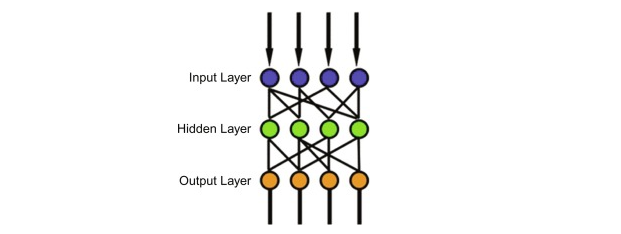
\includegraphics[width=0.8\linewidth, height=0.8\linewidth, keepaspectratio]{image/mul.png}
	
\end{figure}
\begin{equation}
	o_x = G(b_2 + W_2 h_x)
\end{equation}

\begin{equation}
	h_x = \Phi(x) = s(b_1 + W_1 x)
\end{equation}

s vektory zkreslení \( b_1, b_2 \); maticemi vah \( W_1, W_2 \) a aktivačními funkcemi \( G \) a \( s \). Sada parametrů k učení je sada \( \theta = \{W_1, b_1, W_2, b_2\} \). Typické volby pro \( s \) zahrnují tanh funkci s \( \text{tanh}(a) = \frac{e^a - e^{-a}}{e^a + e^{-a}} \) nebo logistickou sigmoidní funkci, s \( \text{sigmoid}(a) = \frac{1}{1 + e^{-a}} \).

\chapter{Využité postupy a technologie}
V průběhu projektu byly využity následující postupy a technologie:

\begin{itemize}
	\item \textbf{Posilované učení (Reinforcement Learning):} Implementace metody Q-learning pro efektivní rozhodování a adaptaci umělé inteligence v dynamických prostředích, což je klíčové pro navigaci v bludišti.
	\item \textbf{Python a PyTorch:} Použití programovacího jazyka Python ve spojení s PyTorch, oblíbeným nástrojem pro strojové učení. PyTorch je významný svým použitím tensorů, které jsou základem pro modelování a trénování neuronových sítí.
	\item \textbf{Raylib v Rustu pro vykreslení prostředí:} Využití knihovny Raylib v programovacím jazyce Rust pro efektivní vykreslení a vizualizaci 2D bludiště, poskytující hladkou grafiku a interakci s herním prostředím.
\end{itemize}

\section{2D bludiště ovládané umělou inteligencí}

\subsection{Vytvoření a interakce s prostředím}
V rámci tohoto projektu je implementováno 2D bludiště, navigované umělou inteligencí. Klíčovou roli v procesu vývoje a tréninku AI modelu hraje PyTorch, pokročilá knihovna pro strojové učení v Pythonu. PyTorch poskytuje efektivní nástroje pro práci s neurálními sítěmi, zvláště díky svým flexibilním a výkonným tensorům.

\subsection{Ovládání bludiště}
Interakce mezi AI a bludištěm je realizována prostřednictvím knihovny pyautogui v Pythonu. Tato knihovna umožňuje AI ovládat herní prostředí simulací klávesových a myšových akcí, což je nezbytné pro dynamické testování a experimenty.
\newpage
\subsection{Vykreslení prostředí}
Bludiště je vykresleno pomocí knihovny Raylib v jazyce Rust, která poskytuje efektivní a snadné prostředky pro tvorbu her a vizualizaci herních prvků. Tento výběr zaručuje hladké a realistické grafické zobrazení prostředí pro AI.
\begin{figure}[h]
	\centering
	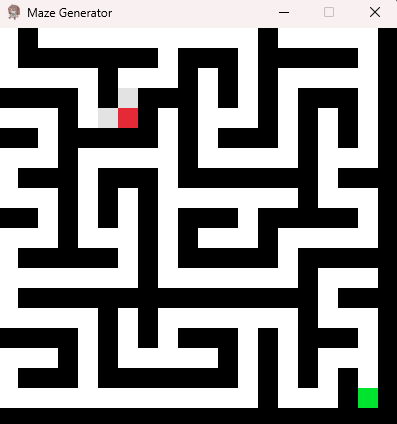
\includegraphics[width=0.3\linewidth, height=0.3\linewidth, keepaspectratio]{image/map.png}
\end{figure}[h]
\subsection{Tensorová reprezentace v PyTorch}
Tensor je základním stavebním kamenem v PyTorch, poskytující mnohovrstevnou, multidimenzionální matici. Tensory v PyTorch slouží jako kontejnery pro data, která jsou zpracovávána a analyzována neuronovými sítěmi. Díky své vysoké efektivitě a flexibilitě jsou tensory nezbytné pro optimalizaci výpočtů a umožňují efektivně manipulovat s velkými datovými sadami.

\begin{figure}[h]
	\centering
	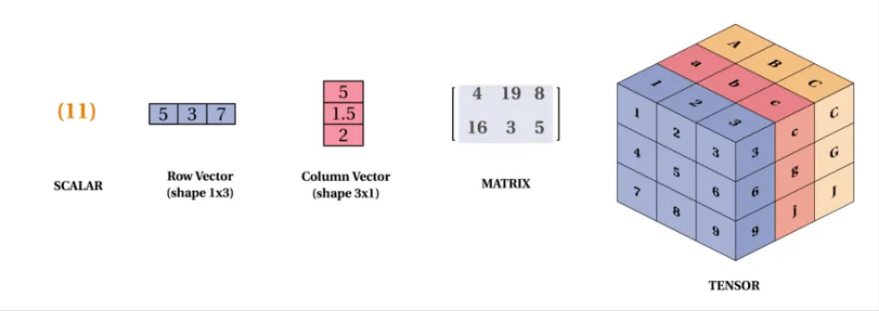
\includegraphics[width=0.8\linewidth, height=0.8\linewidth, keepaspectratio]{image/nazev.png}
\end{figure}[h]

\subsection{Využití tensorů v AI navigaci}
V kontextu AI navigace bludištěm jsou tensory v PyTorch využívány pro reprezentaci a zpracování stavů, akcí a odměn v procesu učení. Tensory umožňují rychlé a efektivní výpočty potřebné pro dynamické aktualizace Q-hodnot v procesu Q-learningu a zajišťují efektivní trénink a optimalizaci neuronových sítí.



\chapter{Řešení problému}

\section{Generování Bludiště pro AI}

Vývoj prostředí pro umělou inteligenci zahrnuje tvorbu bludiště, které AI musí prozkoumat a řešit. Následující fragment kódu v jazyce Rust demonstruje algoritmus pro generování bludiště. Tento algoritmus je základním kamenem pro vytváření dynamických a výzvou bohatých prostředí, ve kterých se AI může učit a rozvíjet.

\lstloadlanguages{rust} % Pokud je toto potřeba, záleží na verzi balíčku listings
\begin{lstlisting}[language=rust, caption={Funkce pro generování bludiště v Rustu}]
fn generate_maze(&mut self, x: usize, y: usize) {
	self.grid[y][x] = 0;
	let mut dirs = [(0, -1), (1, 0), (0, 1), (-1, 0)];
		
	dirs.shuffle(&mut self.rng);
		
	for (dx, dy) in dirs {
		let nx = (x as i32 + dx * 2) as usize;
		let ny = (y as i32 + dy * 2) as usize;
			
	 if nx < GRID_WIDTH as usize && ny < GRID_HEIGHT
	  as usize && self.grid[ny][nx] == 1 {
		self.grid[y.wrapping_add(dy as usize)]
		[x.wrapping_add(dx as usize)] = 0;
		self.generate_maze(nx, ny);
		}
	}
}
\end{lstlisting}


Tento algoritmus využívá rekurzivní způsob k procházení a otevírání cest v mřížce, která reprezentuje bludiště, čímž vytváří cesty a slepé uličky. Výsledná struktura bludiště pak poskytuje komplexní prostředí pro testování a vývoj algoritmů umělé inteligence.


\section{Ukládáni a práce s daty}

Pro ukládání dat o pohybech v bludišti je implementována funkce \texttt{write\_to\_csv}, která přijímá data o pohybech a boolean hodnotu indikující, zda bylo bludiště úspěšně dokončeno. Tato funkce vytvoří CSV soubor a zapíše do něj hlavičku a následně záznamy o jednotlivých pohybech.


\subsection{Implementace funkce write\_to\_csv}

\begin{lstlisting}[language=rust, caption={Funkce pro zápis do CSV souboru}]
	fn write_to_csv(moves_data: &MovesData, is_completed: bool) {
		let file_path = "moves_data.csv";
		let mut file = File::create(file_path);
		
		// Write the header
		writeln!(file, "move;possible_moves;completion_message")
		
		// Process and write moves data to CSV
		for (move_key, possible_moves) in &moves_data.moves {
			// ... (zde pokracuje logika pro zapis dat)
		}
	}
\end{lstlisting}

Tato funkce přepisuje stávající CSV soubor při každém volání, což zajišťuje, že data jsou aktuální. V případě, že je bludiště dokončeno, poslední záznam v CSV bude obsahovat speciální značku indikující úspěšné dokončení.

\newpage
\subsection{Zpracování dat a jejich sledování}

Systém sledování souborů je klíčový pro automatizaci procesu zpracování dat. V našem případě jsme implementovali třídu \texttt{CSVFileMonitor} v Pythonu, která nám umožňuje monitorovat a reagovat na změny v CSV souboru v reálném čase. Tato třída využívá knihovnu \texttt{watchdog}, která poskytuje široké možnosti pro sledování souborového systému, a knihovnu \texttt{csv} pro zpracování CSV souborů. Knihovna \texttt{watchdog} byla vybrána pro svou efektivitu a přenositelnost mezi různými operačními systémy, zatímco \texttt{csv} je standardním nástrojem pro práci s CSV soubory v Pythonu, což zajišťuje snadnou manipulaci s daty.

\subsection{Inicializace a konfigurace monitoru}
Monitorovací třída \texttt{CSVFileMonitor} je inicializována s cestou k sledovanému souboru a adresáři. Může být také konfigurována s callback funkcí, která se vyvolá, když dojde k detekci změny v souboru.

\begin{lstlisting}[language=Python, caption={Inicializace monitoru souboru}]
	class CSVFileMonitor:
	def __init__(self, file_path, directory_path, callback=None):
	self.file_path = file_path
	self.directory_path = directory_path
	self.last_processed_line = None
	self.observer = Observer()
	self.callback = callback
\end{lstlisting}

\subsection{Detekce změn v souboru}
Pro detekci změn v souboru používáme metodu \texttt{has\_file\_updated}, která porovnává čas poslední modifikace souboru s uloženým časem poslední kontroly. Pokud dojde ke změně, aktualizuje se čas poslední kontroly a metoda vrací \texttt{True}, což signalizuje, že soubor byl upraven.

\begin{lstlisting}[language=Python, caption={Detekce změn v CSV souboru}]
	def has_file_updated(self):
	current_modification_time = os.path.getmtime(self.file_path)
	if current_modification_time > self._last_file_modification_time:
	self._last_file_modification_time = current_modification_time
	return True
	return False
\end{lstlisting}

Tato metoda je zásadní pro efektivní sledování souboru bez nepotřebného čtení celého souboru při každém průchodu kontrolní smyčkou. Pouze změny, které jsou skutečně zjištěny, vedou k dalšímu zpracování, čímž se optimalizuje výkon a reaktivita systému.


\subsection{Sledování a reakce na události souborového systému}
Pro sledování událostí souborového systému využíváme knihovnu \texttt{watchdog}. Instance \texttt{Observer} z knihovny je použita k naplánování sledování, což umožňuje spustit předdefinovanou akci vždy, když dojde ke změně ve sledovaném souboru.

\begin{lstlisting}[language=Python, caption={Sledovani a reakce na zmeny souboru}]
	def start(self):
	event_handler = FileSystemEventHandler()
	event_handler.on_modified = lambda event: \
	self.process_file() if event.src_path == self.file_path else None
	self.observer.schedule(event_handler, path=self.directory_path, recursive=False)
	self.observer.start()
\end{lstlisting}

Tato podsekce podrobně popisuje mechanismus sledování a reakce na změny v CSV souboru, který je základem pro dynamické zpracování dat v reálném čase. Výběr knihoven \texttt{watchdog} a \texttt{csv} je zdůvodněn jejich vysokou efektivitou a snadným použitím v Pythonu, což umožňuje flexibilní a robustní řešení pro monitorování souborů.

\subsection{Získání informací o aktuálním stavu hry}
Pro získání důležitých informací o aktuálním stavu hry jsou využívány dvě funkce: \texttt{get\_possible\_moves} a \texttt{get\_completion\_message}.

Funkce \texttt{get\_possible\_moves} vrací seznam možných pohybů v aktuálním kroku hry. Tento seznam je extrahován z posledního zpracovaného řádku CSV souboru a je určen k informování AI o dostupných možnostech pohybu.

\begin{lstlisting}[language=Python, caption={Získání seznamu možných pohybů}]
	def get_possible_moves(self):
	if self.last_processed_line:
	return self.parse_list(self.last_processed_line[1])
	return None
\end{lstlisting}
\newpage
Druhá funkce, \texttt{get\_completion\_message}, zjišťuje, zda bylo bludiště úspěšně dokončeno. Tato informace je také extrahována z posledního řádku CSV souboru a je používána k určení, zda AI dosáhla cíle.

\begin{lstlisting}[language=Python, caption={Zjištění dokončení bludiště}]
	def get_completion_message(self):
	if self.last_processed_line:
	return int(self.last_processed_line[2])
	return None
\end{lstlisting}

Tyto funkce jsou zásadní pro dynamickou interakci AI s prostředím, poskytují nezbytné informace pro rozhodování a strategii hry.



\section{Implementace Algoritmu Q-Learning}

Algoritmus Q-learning je implementován několika zásadními funkcemi, které zajišťují různé aspekty učícího se procesu. Níže jsou detailněji popsány klíčové funkce použité ve skriptu:

\subsection{Funkce Epsilon-Greedy Policy}
\begin{lstlisting}[language=Python]
	def epsilon_greedy_policy(state, valid_moves, epsilon):
	if random.uniform(0, 1) < epsilon:
	action = random.choice(valid_moves)
	print(f"Exploring: Chosen action {action} from {valid_moves}")
	return action
	else:
	valid_q_values = Q_table[state, valid_moves]
	action = valid_moves[torch.argmax(valid_q_values).item()]
	print(f"Exploiting: Chosen action {action} with Q-values {valid_q_values}")
	return action
\end{lstlisting}
Tato funkce rozhoduje mezi prozkoumáním nových možností a využitím stávajících znalostí. Rozhodnutí je založeno na proměnné '\$exploration\_prob\$'. Funkce náhodně vybere akci pro prozkoumání nebo akci s nejvyšší hodnotou Q pro využití znalostí.

\newpage
\subsection{Funkce Provedení Pohybu}
\begin{lstlisting}[language=Python]
	def execute_move(action):
	if action == 0:   # Up
	pyautogui.press('w')
	elif action == 1: # Left
	pyautogui.press('a')
	elif action == 2: # Down
	pyautogui.press('s')
	elif action == 3: # Right
	pyautogui.press('d')
\end{lstlisting}
Tato funkce překládá vybranou akci na příkaz stisku klávesy pomocí 'pyautogui'. Je to způsob, jakým agent interaguje s prostředím - každá akce (0 až 3) odpovídá pohybu v určitém směru.

\subsection{Funkce Získání Dalšího Stavu}
\begin{lstlisting}[language=Python]
	def get_next_state(current_x, current_y, action, valid_moves):
	if action in valid_moves:
	if action == 0:   # Up
	current_y = max(current_y - 1, 0)
	elif action == 1: # Left
	current_x = max(current_x - 1, 0)
	elif action == 2: # Down
	current_y = min(current_y + 1, 18)
	elif action == 3: # Right
	current_x = min(current_x + 1, 18)
	return current_x, current_y
\end{lstlisting}
Funkce vypočítá, kam se agent přesune po provedení akce. Bere v úvahu aktuální pozici (X, Y) a akci, a upravuje pozici agenta v rámci definovaných hranic (např. v 10x10 mřížce).

\newpage
\subsection{Aktualizace Q-Learning}
\begin{lstlisting}[language=Python]
	with torch.no_grad():
		Q_table[current_state, action] = (
		Q_table[current_state, action] + 
		learning_rate * (reward + discount_factor *
		 torch.max(Q_table[next_state]) - 
		Q_table[current_state, action])
		)
\end{lstlisting}
Tento úsek kódu aktualizuje Q-tabulku pomocí algoritmu Q-learning. Hodnoty v Q-tabulce reprezentují odhadovanou odměnu za provedení určitých akcí v určitých stavech. Aktualizace umožňuje agentovi se učit z jeho zkušeností.



	
	\chapter*{Závěr}
	
	V rámci této práce bylo naším hlavním cílem prozkoumat aplikaci Q-learningu, metody posilovaného učení, pro simulaci navigace umělé inteligence v bludišti. Soustředili jsme se přitom na základní principy této metody a její praktickou implementaci v kontextu AI. Praktická demonstrace modelu AI, který řeší bludiště pomocí Q-learningu, odhalila jak obrovský potenciál tohoto přístupu, tak i některé výzvy, které s sebou přináší. Tato práce tak nabízí podrobný pohled na využití posilovaného učení v kontextu řešení konkrétního problému a demonstruje jeho užitečnost v praxi.
	
	
	%% literatura
	\begin{thebibliography}{99}
		\bibitem{neuralNetWiki} WIKIPEDIA. \textit{Umělá neuronová síť} [online]. San Francisco (CA): Wikimedia Foundation, 2021- [cit. 2023-11-11]. Dostupne z: \url{https://cs.wikipedia.org/wiki/Umela_neuronova_sit}
		\bibitem{neuralNetCVUT} REHOR, Václav. \textit{Umělé neuronové sítě} [online]. Praha: ČVUT, 2021 [cit. 2023-11-11]. Dostupné z: \url{https://users.fit.cvut.cz/~rehorto2/otevrena-fakulta/neural-networks.html}
		\bibitem{neuralNetZCU} \textit{Typy umělých neuronových sítí} [pdf]. Plzeň: Západočeská univerzita, 2021 [cit. 2023-11-11]. Dostupné z: \url{https://www.kky.zcu.cz/uploads/courses/nses/2_Typy_umelych_neuronovych_siti-faze_jejich_cinnosti-pouziti.pdf}
		\bibitem{neuralNetMUNI} \textit{Neuronové sítě - jednotlivý neuron} [pdf]. Brno: Masarykova univerzita, 2021 [cit. 2023-11-11]. Dostupné z: \url{https://is.muni.cz/www/98951/41610771/43823411/43823458/Analyza_a_hodnoc/44563149/04Neuronove_site_-_jednotlivy_neuronV1_.pdf}
		\bibitem{PyTorch} \textit{PyTorch} [online]. [cit. 2023-11-11]. Dostupné z: \url{https://pytorch.org}
		\bibitem{ANNVSB} \textit{Popis ANN} [pdf]. Ostrava: VŠB - Technická univerzita Ostrava, 2021 [cit. 2023-11-11]. Dostupné z: \url{http://homel.vsb.cz/~rep75/Predmety/AI/ANN/BackPropagation/Popis%20ANN.pdf}
		\bibitem{OpenAI} OPENAI. \textit{OpenAI Research and Technology} [online]. San Francisco (CA): OpenAI LLP, 2023- [cit. 2024-01-10]. Dostupné z: \url{https://openai.com/research/}
		\bibitem{GoogleAI} GOOGLE AI. \textit{Google AI} [online]. Mountain View (CA): Google LLC, 2023- [cit. 2024-01-10]. Dostupné z: \url{https://ai.google/}
		\bibitem{MIT_AI_Agents} 
		GORDON, R. \textit{AI agents help explain other AI systems}. San Francisco (CA): MIT Schwarzman College of Computing, 2024-01-03. Dostupné z: \url{https://computing.mit.edu}
		
		\bibitem{MIT_Compositional_Foundation_Models} 
		AJAY, A. and AGRWAL, P. \textit{Compositional Foundation Models for Hierarchical Planning}. Massachusetts: Massachusetts Institute of Technology, 2023. Dostupné z: \url{https://arxiv.org}
		
		\bibitem{MIT_HiP_Project} 
		AJAY, A. and AGRWAL, P. \textit{HiP project}. Massachusetts: Computer Science and Artificial Intelligence Laboratory, MIT, 2023. Dostupné z: \url{https://hierarchical-planning-foundation-model.github.io}
		
		\bibitem{MIT_Multiple_AI_Models} 
		MIT NEWS. \textit{Multiple AI models help robots execute complex plans more transparently}. Massachusetts: Massachusetts Institute of Technology, 2024-01-03. Dostupné z: \url{https://news.mit.edu}
		
	\end{thebibliography}
	

\end{document}